\documentclass[tikz]{standalone}


\tikzstyle{node}=[draw=#1,fill=#1!20]

\newcommand{\vertex}[6]{\node[shape=circle,fill=black, scale=0.5,label=#1:{#2},label=#5:{\tiny\texttt{\color{blue}#6}},#4] (#3)  {};}
\newcommand{\myedge}[4]{ \draw[->] (#1) edge node[#2] {#3} (#4);}
\usetikzlibrary{automata,calc}
\tikzset{
	initial text=\(\ast\),
}


\begin{document}
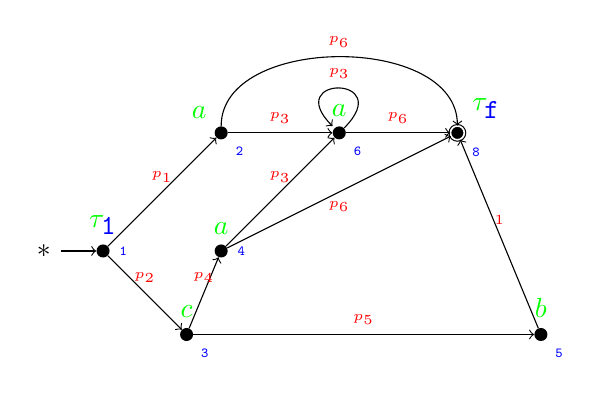
\begin{tikzpicture}[align=center,node distance=3cm]
    % equidistant points and arc
    \vertex{above}{$\color{green}\tau_\texttt{\color{blue}1}$}{s}{initial}{right}{1}
    \vertex{above}{$\color{green}a$}{a2}{right of=s}{right}{4}
    
    %\node[above right of=s] (bp) {};
    \vertex{above left}{$\color{green}a$}{bp2}{above of=a2}{below right}{2}
    \vertex{above}{$\color{green}a$}{b1}{right of=bp2}{below right}{6}
    
    
    \vertex{above}{$\color{green}c$}{b2}{below right of=s}{below right}{3}
    \node[ right of=b2] (e2) {};
    
    %\node[shape=circle,fill=black, scale=0.5,label=left:{\color{green}$a$},label=below right:{\tiny\texttt{\color{blue}4}}] (a2) at ($(e2)!0.5!(bp2)$) {};
    
    \vertex{above}{$\color{green}b$}{b}{right of=e2}{below right}{5}
    \vertex{above right}{$\color{green}\tau_\texttt{\color{blue}f}$}{f}{right of=b1,accepting,state,scale=0.4}{below right}{8}
    
    %
    \myedge{s}{above}{$\scriptscriptstyle{\color{red}p_1}$}{bp2}
    \myedge{bp2}{above}{$\scriptscriptstyle{\color{red}p_3}$}{b1}
    \draw (bp2) edge [->,bend left=90] node [midway,above] {$\scriptscriptstyle{\color{red}p_6}$} (f);
    
    \myedge{s}{above}{$\scriptscriptstyle{\color{red}p_2}$}{b2}
    \myedge{b2}{above}{$\scriptscriptstyle{\color{red}p_4}$}{a2}
    \myedge{a2}{above}{$\scriptscriptstyle{\color{red}p_3}$}{b1}
    \myedge{a2}{below}{$\scriptscriptstyle{\color{red}p_6}$}{f}
    \myedge{b2}{above}{$\scriptscriptstyle{\color{red}p_5}$}{b}
    \myedge{b}{above}{$\scriptscriptstyle{\color{red}1}$}{f}
    %\myedge{f}{right}{$\scriptscriptstyle{\color{red}1}$}{bk}
    \myedge{b1}{above}{$\scriptscriptstyle{\color{red}p_6}$}{f}
    
    \draw[->,shorten >=1pt] (b1) edge [in=135,out=45,loop,looseness=20] node [above] {$\scriptscriptstyle{\color{red}p_3}$} (b1);
\end{tikzpicture}

\end{document}
